%% ---------------------------------------------------------------------------------------------------------------------

\chapter{Background}\label{ch:background}

This chapter presents background information that is necessary for this thesis.
First, the \unsafe{} \acrshort{API} as well as slices and strings in Go is discussed.
Then, Go memory management is introduced, and exploit techniques and mitigations are presented.
After this, Go dependency management is covered, and the chapter concludes with concepts about static code analysis.


%% ---------------------------------------------------------------------------------------------------------------------

\section{Go Unsafe API}\label{sec:background:unsafe-api}

The Go \unsafe{} package~\footnote{\url{https://golang.org/pkg/unsafe}} is an application programming interface
(\acrshort{API}) that allows developers to use raw pointers with all their benefits and dangers.
As such, it offers an escape hatch to circumvent safety measures provided by Go.
Listing~\ref{lst:unsafe-api} shows the functions and types included in the \unsafe{} package.

\begin{lstlisting}[language=Golang, label=lst:unsafe-api, caption=\textit{Unsafe} package API]
package unsafe

type Pointer

func Alignof(x ArbitraryType) uintptr
func Offsetof(x ArbitraryType) uintptr
func Sizeof(x ArbitraryType) uintptr
\end{lstlisting}

There are \checkNum{three} functions \textit{Sizeof}, \textit{Alignof}, and \textit{Offsetof} (Lines~5--7),
as well as the type \textit{Pointer} (Line 3).
The \textit{unsafe.Pointer} is the most significant package member with respect to the possibilities that it offers.
It is a pointer type that is exempt from the restrictions that normally apply in order to improve memory safety.
In particular, unsafe pointers can be converted to and from any other pointer type, allowing arbitrary casts between
any type.
Furthermore, they can be converted to and from \textit{uintptr} values, which is an integer type with sufficient size
to store pointers on the specific target architecture of the program.
Since \textit{uintptr} values behave like normal integer variables, they can be used in arithmetic expressions.
Therefore, unsafe pointers can also be used to achieve pointer arithmetic.
With \textit{unsafe.Pointer}, developers can achieve the same flexibility as with raw \textit{void*} pointers in C.

Listing~\ref{lst:unsafe-examples} shows examples of both \textit{unsafe.Pointer} features.
The \textit{floatToBits} function (Line~3) illustrates how the variable \textit{x} of type \textit{float32} is first
cast to an unsafe pointer and then to a value of type \textit{int} (Line~4).
Since the unsafe conversion rules only allow arbitrary casts between any pointer type, \textit{x} is first converted
into a pointer value and the resulting \textit{int} pointer is dereferenced before returning the final value.
This conversion yields the raw bits of the floating point value stored using the IEEE 751 format.
It would be impossible using the normal Go conversion rules because \textit{float32} and \textit{int} are incompatible
types.
The \textit{secondByte} function (Line~7) shows how pointer arithmetic is used to manually iterate over an array type.
The function expects an array of size five bytes and returns the second byte.
Instead of direct indexing, it achieves this by obtaining the address of the array as a \textit{uintptr} value, adding
1 and then casting the resulting address to a \textit{byte} value, again taking care of dereferencing the resulting
pointer type (Line~8).

\begin{lstlisting}[language=Golang, label=lst:unsafe-examples, caption=Usage examples of the Go \textit{unsafe} API]
import "unsafe"

func floatToBits(x float32) int {
    return *(*int)(unsafe.Pointer(&x))
}

func secondByte(b [5]byte) byte {
    return *(*byte)(unsafe.Pointer(uintptr(unsafe.Pointer(&b)) + 1))
}
\end{lstlisting}

%It is important to note that while \textit{unsafe.Pointer} is a pointer type, \textit{uintptr} is not.
%This means that addresses that are stored in variables of type \textit{uintptr} are not treated as references by the
%garbage collector, and thus values referenced by it can get freed although there are still live references.
%Possible consequences of this are described in Chapter~\ref{ch:unsafe-security-problems}.
%Other dangers include that accessing raw bytes of data structures exposes low-level implementation details such as
%the alignment of structure fields to word-bound addresses, which can change with future versions of the Go compiler or
%runtime and thus break programs when they are not carefully updated later on.
%In general, using the \unsafe{} package must be done with caution and should be avoided whenever possible.

The other functions of the \unsafe{} packages are evaluated at compile time and can be used to gain knowledge about
the size, alignment, or offset of a field in a structure type relative to the start of the structure.
These can be necessary when dealing with the direct byte representations of structure types such as when implementing
network protocols or device drivers.
In this thesis the term \unsafe{} usage refers to all members of the \unsafe{} package as well as the slice and string
header structures that are described in the next section.


%% ---------------------------------------------------------------------------------------------------------------------

\section{Slices and Strings in Go}\label{sec:background:slices}

Slices in Go (e.g. the \textit{[]byte} type) are views on arrays~\footnote{\url{https://blog.golang.org/slices}}.
They are a data type consisting of an underlying memory area storing the array data, as well as information about length
and capacity of the slice.
The Go runtime takes care that there are no accesses outside the slice bounds.
The length indicates how many elements are contained in the slice, and the capacity denotes the allocated space in
memory.
The capacity is always equal or greater than the length.
If it is greater, then elements can be added by increasing the length without allocating new memory.
Only if the length is equal to the capacity and a new element is added, the Go runtime allocates a new, bigger
underlying memory array and copies the existing data.
When a subset of the slice is taken by specifying start and end indices, then a new slice is created that uses the same
underlying data array as the original one, and might have a capacity longer than its length if there are further
elements in the original slice after the end of the newly-taken subslice.

Strings in Go are read-only \textit{[]byte} slices~\footnote{\url{https://blog.golang.org/strings}}.
Usually they are encoded in UTF-8, but this is not required.
The length of a string is always the number of bytes needed to store its encoded form, which is often not the same as
the number of characters in the string.
Strings are immutable because string literals are placed in a constant data section of the binary when the code is
compiled, meaning they are usually located within a read-only memory page at runtime and mutating them would cause
the program to receive a segmentation fault signal and crash.
Since strings can not be changed, there is no need to have a capacity that is different from the length, therefore there
is no capacity information available for strings.

It is possible to access the internal structure of slices and strings by casting them to a slice or string header
representation using the \unsafe{} \acrshort{API}.
Listing~\ref{lst:reflect-header-types} shows the \acrshort{API} of these header types, which are part of the Go
\textit{reflect} package~\footnote{\url{https://golang.org/pkg/reflect}}.

\begin{lstlisting}[language=Golang, label=lst:reflect-header-types, caption=Reflect slice and string header types and API]
package reflect

type SliceHeader struct {
    Data uintptr
    Len int
    Cap int
}

type StringHeader struct {
    Data uintptr
    Len int
}
\end{lstlisting}

As the name suggests, slices correspond to the \textit{SliceHeader} type (Line~3), while strings are associated with the
\textit{StringHeader} type (Line~9).
The \textit{Len} fields (Lines~5 and~11) denote the current length of the slice or string, and the \textit{SliceHeader}
type has an additional \textit{Cap} field (Line~6) for the slice capacity.
The reference to the underlying data array is a \textit{uintptr} value in both types (\textit{Data} in Lines~4 and~10).
This means that it is not inherently a pointer type, instead it stores the plain address of the array.
However, the Go runtime recognizes slices and strings and treats their \textit{Data} field like a pointer as a special
case.

Slices are different from array or buffer types like \textit{[10]byte}, which have a fixed length.
There is no way to grow an array by appending more data than it can store.
Furthermore, the Go type system makes the array length a fundamental property of the type, which means that there can
not be an implicit conversion between arrays of different lengths.
In contrast, slices store their length in a variable and are not treated differently by the type system depending on
their length.


%% ---------------------------------------------------------------------------------------------------------------------

\section{Memory Management in Go}\label{sec:background:memory}

The Go programming language uses automatic memory management, which means that developers do not need to manually
allocate and free memory for data structures, instead a value is simply declared and the compiler adds the code to
properly allocate the appropriate space in memory.
This section first describes how the stack and heap are used in Go, and then introduces garbage collection and escape
analysis.


%% ---------------------------------------------------------------------------------------------------------------------

\subsection{Stack and Heap}\label{subsec:background:memory:stack-heap}

The available memory addresses that an application can access are divided into logical sections.
Go programs always at least use a program code, stack, and heap section, although there can be more.
Figure~\ref{subfig:memory:memory-layout} shows an illustration of the distribution of these sections in the address
space.

\begin{figure}[htp!]
    \centering

    \begin{subfigure}[t]{0.45\textwidth}
        \centering
        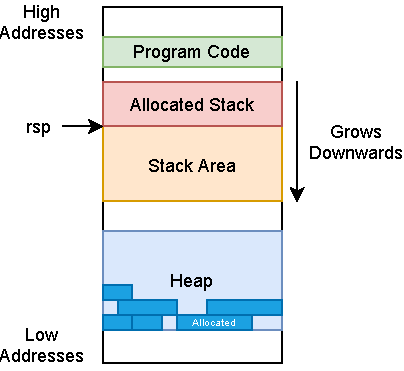
\includegraphics[height=5.5cm]{assets/figures/chapter2/memory-layout.pdf}
        \caption{Process memory layout}
        \label{subfig:memory:memory-layout}
    \end{subfigure}
    \begin{subfigure}[t]{0.45\textwidth}
        \centering
        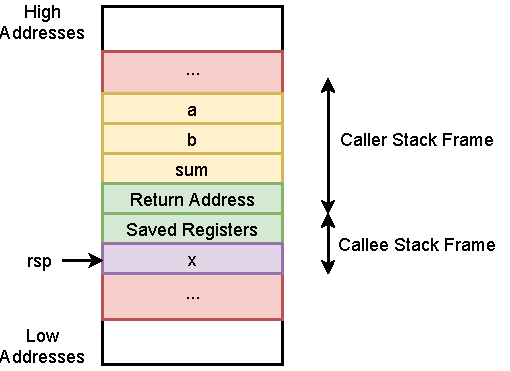
\includegraphics[height=5.5cm]{assets/figures/chapter2/stack-frame.pdf}
        \caption{Simplified stack frame layout for function in Listing~\ref{lst:stack-example-function}}
        \label{subfig:memory:stack-frame}
    \end{subfigure}

    \caption{Go memory and stack frame layout}
    \label{fig:memory-stack}
\end{figure}


The program code (shown in green) is loaded at a relatively low address.
Then, the stack area (red and orange) follows, and finally the heap section (shown in blue) is located at higher
addresses.
The stack area is used to store data that is associated with individual functions, and will be needed only as long as
the function runs~\cite{ferres2010}.
In contrast, the heap contains values with a lifetime that is longer than the execution of a specific function, for
example global variables.
In Go, developers do not actively decide whether a variable is allocated on the stack or heap, this is done by the
compiler.

The stack pointer \textit{rsp} (this name is specific to the \textit{amd64} architecture, but the concept applies to
other architectures as well) is a register that contains the address of the last value that was allocated on the stack.
As shown in Figure~\ref{subfig:memory:memory-layout}, it thus marks the border of the used part of the stack area.
When new values are stored (pushed) on the stack, the stack pointer is decremented and the data is stored at the
resulting new address in \textit{rsp}.
Therefore, the stack grows downwards, from high to low addresses.

Data on the stack is organized in frames.
When a function is called, a new stack frame is created for it.
Figure~\ref{subfig:memory:stack-frame} shows a visualization of this.
It presents the stack after calling the \textit{add} function in Listing~\ref{lst:stack-example-function}.

\begin{lstlisting}[language=Golang, label=lst:stack-example-function, caption=Example function to illustrate Go stack frames]
func add(a , b int) (sum int) {
    x := a + b
    sum := x + 42
    return sum
}
\end{lstlisting}


In Go, function parameters and return values are both passed entirely on the
stack~\footnote{\url{https://go.googlesource.com/proposal/+/master/design/27539-internal-abi.md}}.
Therefore, the parameters \textit{a} and \textit{b}, as well as the return value \textit{sum} (declared in Line~1) are
pushed onto the stack by the caller function.
They are shown in yellow in Figure~\ref{subfig:memory:stack-frame}.
The last value that gets pushed into the caller frame is the address of the next instruction to execute after the callee
function returns.
It is called return address or return instruction pointer (\acrshort{RIP}) and shown in green.
Then, the new stack frame for the callee begins with the CPU register contents at the function call time.
These are stored on the stack so that they can be restored to the original values before returning back to the caller.
They are shown in green as well in Figure~\ref{subfig:memory:stack-frame}.
After this, local variables of the callee function that do not surpass its lifetime are pushed to the stack.
In this case, there is the variable \textit{x} (Line~2 in Listing~\ref{lst:stack-example-function}), which is shown in
purple in Figure~\ref{subfig:memory:stack-frame}.
The \textit{sum} variable (Line~3) is not pushed to the callee stack frame, because since it is a return value it was
already placed in the caller stack frame.
When the function \textit{add} returns, the stack pointer \textit{rsp} will be incremented up to the \textit{sum} value
to destroy the callee stack frame, and the CPU will jump to the return address that was stored on the stack.

In constrast, data on the heap is organized in chunks~\cite{ferres2010}.
There can be several allocated chunks of data on the heap, and they are not necessarily adjacent.
Figure~\ref{subfig:memory:memory-layout} shows used heap areas in a darker shade of blue.
Adding data to the heap requires calling special allocation functions that are provided by the runtime, which in the
case of Go is done automatically by the compiler.
Furthermore, memory on the heap must be freed when it is not longer used, otherwise the program will run out of usable
heap space eventually.
Therefore, storing data on the heap has more overhead than the stack, because deallocation on the stack is done with a
single addition when destroying an entire stack frame.


%% ---------------------------------------------------------------------------------------------------------------------

\subsection{Garbage Collection (GC)}\label{subsec:background:memory:gc}

The Go runtime uses a move-and-sweep garbage collector (\acrshort{GC}) to free unused heap memory~\cite{sibiryov2017}.
It is triggered by one of two conditions, either when the heap usage has increased to a specific size (usually when the
usage has doubled since the last \acrshort{GC} run), or after a fixed time has passed without any \acrshort{GC} runs.
Figure~\ref{fig:gc-visualization} shows a visualization of the marking phase in a \acrshort{GC} run.
Rounded boxes represent variables, rectangular boxes are allocated values on the heap, and arrows indicate references
from pointer types to their targets.

\begin{figure}[htp!]
    %\vspace{2mm}
    \centering
    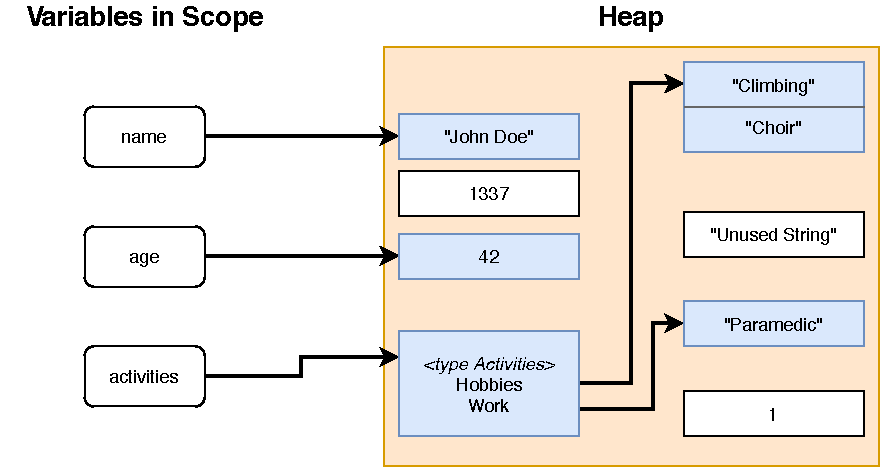
\includegraphics[width=0.6\textwidth]{assets/figures/chapter3/gc-visualization.pdf}
    \caption{Garbage Collector Visualization}
    \label{fig:gc-visualization}
    %\vspace{-10pt}
\end{figure}


The \acrshort{GC} takes all variables that are present in the scope of the program and marks them as live.
These variables can be either on the stack, which is not managed by the \acrshort{GC}, or on the heap.
In this case, there are the \textit{name}, \textit{age}, and \textit{activities} variables with the values
\textit{"John Doe"}, \textit{42}, and \textit{Activities}, which are shown in blue in Figure~\ref{fig:gc-visualization}.
Then, it recursively follows all pointer types within live variables and marks their target values as live, too.
This concerns the values \textit{"Climbing"}, \textit{"Choir"}, and \textit{"Paramedic"}.
However, the values \textit{1337}, \textit{"Unused String"}, and \textit{1} are not reachable from any pointer variables
in scope, and therefore are not marked.
They are shown in white in the figure.

After this marking phase has completed, the sweep phase frees all memory that is not marked as live.
Finally, the markings are reset and a new \acrshort{GC} run can be triggered.

Using a \acrshort{GC} improves memory safety in Go because without explicit deallocations, the risk of dereferencing
pointers that have already been freed (\textit{use-after-free}) is reduced.
The Go GC runs concurrently with all other threads of a program.
During the mark phase, it briefly stops the execution of the other threads to ensure a consistent view on all live
heap values.
The sweep phase is executed in parallel to the other threads.


%% ---------------------------------------------------------------------------------------------------------------------

\subsection{Escape Analysis (EA)}\label{subsec:background:memory:ea}

Escape analysis (\acrshort{EA}) is a technique to decide whether a variable can be placed on a function's stack or needs
to be allocated on the heap.
It is used by the Go compiler when a variable is declared.
Go prefers to allocate on the stack if possible, because there is no explicit deallocation step needed to free the value
there.
Instead, the stack frame is removed entirely when the function returns.

In \acrshort{EA}, a value is said to escape if references to it can live longer than the lifetime of the current
function.
If it does escape, then it needs to be allocated on the heap so that when the function has terminated, references that
still exist can continue to access the memory even though the stack frame has vanished.
Otherwise, it can be placed on the stack.

The \acrshort{EA} analysis employed by the Go compiler works by checking for each variable that is declared in a
function whether a reference to it is stored in another value or passed to another function.
If there is a reference stored in another object, this object has to be checked too, and if it escapes then so does the
original variable.
The same is true for functions.
If the variable gets passed to another function then the \acrshort{EA} algorithm transitively looks into that function
and determines if the value escapes there.
If it does, then it must also be treated as an escaped value in the original function.
Finally, if the function returns a reference to the variable then it obviously escapes as well.


%% ---------------------------------------------------------------------------------------------------------------------

\section{Exploit Techniques and Mitigations}\label{sec:background:exploit-techniques}

This section briefly explains common exploit techniques and mitigations against them.


%% ---------------------------------------------------------------------------------------------------------------------

\subsection{Buffer Overflow}\label{subsec:background:exploit-techniques:buffer-overflow}

A frequent security vulnerability related to memory safety is the buffer overflow~\cite{larochelle2001}.
It happens when a buffer variable, for example a slice, is too short for the data that is written to it, causing the
data to overflow into and overwrite adjacent memory.
Overflows can happen anywhere in the memory, however a common source of security problems are stack-based buffer
overflows.
When a buffer variable is placed on the stack and too much data gets written to it, the data will be written to higher
memory addresses, which means after overwriting the other local variables and saved registers they can cause the saved
return address to get changed.
When an attacker can control the data that is placed there, they can change the program flow by carefully choosing the
address that the CPU jumps to after the current function returns.

Figure~\ref{fig:stack-smashing-payload} shows a visualization of an example input data used to execute arbitrary code
by overwriting the saved return address.
This is called \textit{stack smashing}~\cite{smith1997}.
First, a arbitrary data is written to fill up the buffer and any adjacent local variables up to the address of the
saved return address.
Next, the desired new return address is written (\acrshort{RIP}).
This will replace the original, correct address.
By using the address of the following data that gets written to the stack, the program control flow can be redirected to
attacker-controlled code.

\begin{figure}[htp!]
    %\vspace{2mm}
    \centering
    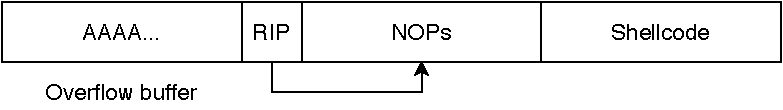
\includegraphics[width=0.8\textwidth]{assets/figures/chapter2/stack-smashing-payload.pdf}
    \caption{Stack smashing payload to inject exploit code}
    \label{fig:stack-smashing-payload}
    %\vspace{-10pt}
\end{figure}


Since stack addresses can be slightly unpredictable in practice, for example because environment variables with
different lengths might be located on the stack, a \textit{NOP-slide} can be used to make the exploit more robust.
\textit{NOP}, or \textit{no-op}, is a machine instruction that does nothing at all, the processor continues with the
following instruction.
A \textit{NOP slide} then is a series of such instructions~\cite{vallentin2007}.
Using this, it is sufficient to overwrite the return instruction pointer with an address somewhere within the
\textit{NOP} instructions to make the processor go through all remaining of them until it reaches the exploit code,
similar to sliding down a slope.
Thus, the address does not have to match the exact start of the payload code anymore, instead it can have a tolerance.
In Figure~\ref{fig:stack-smashing-payload}, the pointer from the overwritten return instruction pointer (\acrshort{RIP})
points into the middle of the \textit{NOP slide}.
After it, the code that the attacker wants to execute is written onto the stack.


%% ---------------------------------------------------------------------------------------------------------------------

\subsection{Data Execution Prevention (DEP)}\label{subsec:background:exploit-techniques:dep}

Data execution prevention (\acrshort{DEP}) is a mitigation technique to prevent the execution of code on the
stack~\cite{gao2013}.
With \acrshort{DEP}, memory pages can either be executable or writable, but not both.
Pages that contain the stack are marked as non-executable.
This achieves improved security because an attacker can not simply write code to the stack using a buffer overflow as
described in the previous section and then execute it.
Modern operating systems use \acrshort{DEP} by default~\cite{davi2011}.


%% ---------------------------------------------------------------------------------------------------------------------

\subsection{Address Space Layout Randomization (ASLR)}\label{subsec:background:exploit-techniques:aslr}

To work around \acrshort{DEP}, attackers can reuse existing functions in the binary, because these are located on
executable (but not writable) memory pages.
However, this can be mitigated using Address Space Layout Randomization (\acrshort{ASLR}).
This technique loads dynamically-linked libraries into random memory positions to avoid having predictable function
addresses~\cite{marco2014}.
Thus, attackers can not use code that is part of standard libraries as a target of control flow redirection because
they can not know the exact address of the desired function.
\acrshort{ASLR} does however not apply to statically-linked code, which the Go compiler mostly creates.


%% ---------------------------------------------------------------------------------------------------------------------

\subsection{Return Oriented Programming (ROP)}\label{subsec:background:exploit-techniques:rop}

Return-oriented programming (\acrshort{ROP}) is a specific technique for reusing code that suggests jumping to very
small so-called gadgets, which are sequences of two or few more machine instructions that do not modify the stack
pointer register and end with a return instruction~\cite{roemer2012}.
With these properties, gadgets can be chained because after the execution of a fragment the return instruction fetches
the next address to jump to from the stack, which the attacker can control when they exploit a buffer overflow
vulnerability.
Depending on the available \acrshort{ROP} gadgets, the attacker can therefore concatenate them and thus write a program
with a limited set of assembler instructions available.
Often, there are enough gadgets present in the program code to form a set that together is Turing complete, thus
arbitrary behaviour can be induced from it.
The Go standard library is very large and thus provides many available gadgets.
This makes exploiting a buffer overflow, once it exists in a Go program, sometimes even easier than in a C program where
an attacker might have to work around \acrshort{ASLR}, for example.


%% ---------------------------------------------------------------------------------------------------------------------

\section{Dependency Management in Go}\label{sec:background:dependencies}

To break code into logical units that can be maintained separately and allow reusing them, Go offers a dependency
management system.
The smallest possible unit is a Go package.
A package can contain one or more source code files which must all be in the same directory.
It has a name which should match the name of the directory containing the source files.
There can not be more than one package in the same folder.
Identifiers such as function and variable names must be unique in the scope of the same package and can be accessed
directly.
Therefore, developers can split their code into individual code files without restrictions to organize a single package.
When accessing code in a different package, the package name must be used as prefix in front of the identifier name.
Furthermore, the package must be imported using an \textit{import} statement at the beginning of the file.
Package imports are valid only within a file, not a whole package, and thus must be repeated in all files that access
an external package.
It is only possible to access exported fields from another package, which is indicated by starting the identifier with
a capital letter.
When importing the package, it is necessary to specify the complete path to the package, the name is not sufficient on
its own.
The import path is made up of the directory tree leading to the package directory, separated by forward slashes.
For example, a valid import path would be \textit{my-application/storage/database}.

To allow sharing code with other developers and implementing reusable libraries, it is possible to download external
packages using the \textit{go get} command, which can fetch packages using the web protocol \acrshort{HTTP}, Git, or
other means.
The import path then usually begins with a \acrshort{DNS} host name such as \textit{github.com}, which hosts the package
code.
This host part is called \textit{registry}.


%% ---------------------------------------------------------------------------------------------------------------------

\subsection{GOPATH and GOROOT}\label{subsec:background:dependencies:gopath}

Before the release of Go \checkNum{1.13}, packages that were fetched using \textit{go get} were stored in the
\textit{GOPATH} directory~\footnote{\url{https://golang.org/doc/gopath_code.html}}.
Furthermore, there exists the \textit{GOROOT} directory, which is similar to \textit{GOPATH} but contains the Go
standard library packages instead of manually downloaded packages.
Environment variables point to these folders, and the Go compiler uses them to get the sources of packages that are not
part of the current project.

This architecture provided a simple way of downloading and using external packages.
However, a serious drawback is that it does not allow to specify a version of the imported package.
Therefore, it is very hard to publish stable libraries because developers can not depend on an old version of the
library, and it is not possible to use different versions of the same package next to each other.


%% ---------------------------------------------------------------------------------------------------------------------

\subsection{Go Module System}\label{subsec:background:dependencies:modules}

Starting with the release of Go \checkNum{1.11}, the development of the module system has fixed this by introducing a
new unit of code organization~\footnote{\url{https://blog.golang.org/using-go-modules}}.
It is stable and the default since Go \checkNum{1.13} in \checkNum{September 2019}.
Modules contain one or more packages, and have a name and import path similar to packages, which can in fact be the name
of a root package in the module.
Furthermore, modules are required to be available as a revision control repository like Git and are versioned.
Downloaded modules are placed in a subdirectory of \textit{GOPATH}, the \textit{module path}.

A project can define dependencies to specific versions of other modules, which resolve to the packages imported in the
code.
Thus, it is possible to require a specific version of an external package.
Dependencies can be transitive, because imported modules can have dependencies to other modules themselves,
forming a dependency tree.
Figure~\ref{fig:dependency-model} shows an example of the relations between the different units of code organization
used in Go.
The \textit{github.com/example/example} module is the main application module and its current version is
\textit{v2.0.0}.
It contains three separate packages \textit{A}, \textit{B}, and \textit{C}, all of which are composed of individual Go
source files.
The module depends upon two other modules \textit{X} and \textit{Y}, both of which are imported with a specific version.
These again contain one or more packages with source files, and further depend on more modules.
The \textit{Y} module is effectively imported in two different versions, \textit{v1.0.1} and \textit{v5.3.0}, so both
their sources will be compiled and included in the resulting binary.

\begin{figure}[htp!]
    %\vspace{2mm}
    \centering
    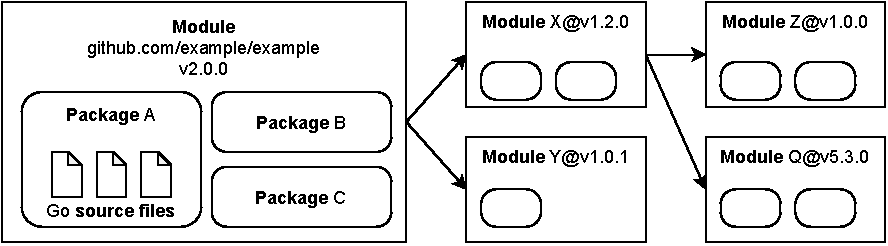
\includegraphics[width=\textwidth]{assets/figures/chapter2/dependency-model.pdf}
    \caption{Dependency management model used by Go}
    \label{fig:dependency-model}
    %\vspace{-10pt}
\end{figure}


Projects lock their dependencies including versions in a file called \textit{Go.mod}.
When the code is built, the Go compiler toolchain will automatically figure out which modules need to be downloaded and
get the code.


%% ---------------------------------------------------------------------------------------------------------------------

\section{Static Code Analysis}\label{sec:background:static-code-analysis}

Static code analysis describes techniques that examine source code for particular properties, such as code metrics or
the presence of specific bugs, without running the program.
In the last point, it is different from dynamic code analysis which executes the code and employs runtime checks.
Using static code analysis, it is possible to automatically test if the source code matches certain expectations.
Based on the level of abstraction that an analysis tool is looking at, it can be classified into lexical, syntactic,
or semantic analysis.
Lexical analysis deals with the source code as text, with the most common purpose being coding style enforcement.
For syntactic analysis, the code is parsed to obtain an abstract syntax tree (\acrshort{AST}), which allows for example
to do type checking and reporting code metrics such as the cyclomatic complexity or McCabe metric~\cite{watson1996}.
Finally, semantic analysis also takes care of the control and data flow, which describe what statements in the code can
be executed in which order and how data is being transferred between variables.
This allows for example to detect unused or dead code, or detect whether a variable is used before it is initialized.
To do this, a control flow graph (\acrshort{CFG}) is used.


%% ---------------------------------------------------------------------------------------------------------------------

\subsection{Abstract Syntax Tree (AST)}\label{subsec:background:static-code-analysis:ast}

Source code of programming languages is a formal language that follows a grammar, which is its syntax.
Syntactically valid programs are words in the formal language and can be represented as the tree of grammar rules used
to construct the word.
This is called the abstract syntax tree (\acrshort{AST}) of the program.

\begin{figure}[htp!]
    %\vspace{2mm}
    \centering
    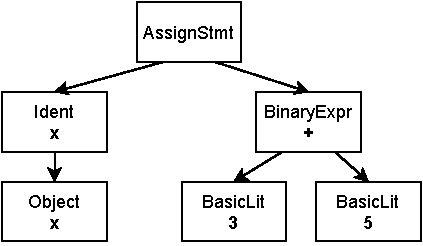
\includegraphics[width=0.5\textwidth]{assets/figures/chapter2/ast.pdf}
    \caption{Abstract syntax tree visualization for source code "x := 3 + 5"}
    \label{fig:ast}
    %\vspace{-10pt}
\end{figure}


Figure~\ref{fig:ast} shows an example \acrshort{AST} for a code fragment of just one statement, which is
\textit{x := 3 + 5}.
A grammar construction of the programming language syntax begins with a start symbol, such as \textit{AssignStmt} in
this case.
It can have children, which are recursively substituted for concrete values.
In Figure~\ref{fig:ast}, the right hand side of the assignment is an addition, an instance of a binary expression, with
basic integer literals 3 and 5 used for the addition.
The \acrshort{AST} shows the composition of the source code into logical units of growing size, with the leafs being
identifiers, literals, or any other nodes that do not contain further children, such as an empty return statement for
example.

To obtain the \acrshort{AST}, it is possible to use the parser bundled with the language's compiler.
An advantage of running static analysis steps on the \acrshort{AST} is that it is independent from any concrete lexical
representation such as white space.
Identifier names can also be easily replaced by different names in the abstract representation, which makes the
\acrshort{AST} suitable for name refactoring operations or recognizing specific types even if they are aliased in the
source code.


%% ---------------------------------------------------------------------------------------------------------------------

\subsection{Control Flow Graph (CFG)}\label{subsec:background:static-code-analysis:cfg}

In contrast, the control flow graph (\acrshort{CFG}) is not purely based on syntax anymore, but needs semantic analysis
to be constructed.
It is a directed graph showing possible execution paths through code segments.
It can contain cycles and is not necessarily connected (neither strongly nor weakly).
Nodes in the control flow graph denote logical pieces of the source code in the sense that they form a unit of
execution.
They can be seen as an atomic step of computation.
While \acrshort{CFG} nodes are also nodes in the \acrshort{AST}, there are \acrshort{AST} nodes that are not a
\acrshort{CFG} node.
Edges in the \acrshort{CFG} represent all possible paths of execution.
An example of a \acrshort{CFG} can be seen in Figure~\ref{fig:cfg}.
It shows the simple loop \textit{for x < 5 \{ x += 1 \}}.

\begin{figure}[htp!]
    %\vspace{2mm}
    \centering
    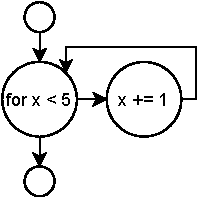
\includegraphics[width=0.25\textwidth]{assets/figures/chapter2/cfg.pdf}
    \caption{Control flow graph for source code "for x < 5 \{ x += 1 \}"}
    \label{fig:cfg}
    %\vspace{-10pt}
\end{figure}


There are two logical steps of execution in this code example.
After any previous code is executed and control flows to the \textit{for} loop, first the loop condition \textit{x < 5}
is checked.
Then, there are two outgoing edges on the node because the condition can be either true or false.
If it is true, then control flows to the assignment node representing the \textit{x += 1} statement.
That node then has an edge back to the loop condition node to check whether the loop should be run again.
Otherwise, the code following behind the loop is executed.

Such a \acrshort{CFG} is an excellent tool to detect dead code, which would be represented by an isolated or unreachable
connectivity component in the graph.
Furthermore, using node annotations that indicate whether variables are read or assigned, it is possible to detect
control flow anomalies such as \textit{read-before-write}, which would show that a variable is used before it is
initialized.
It is also useful to detect where a variable is assigned for the last time before a particular statement, thus what
value it has at the time of execution of that statement.


%% ---------------------------------------------------------------------------------------------------------------------

\subsection{Go Linters \toolVet{} and \toolGosec{}}\label{subsec:background:static-code-analysis:linters}

There are a number of existing static code analysis tools for the Go programming language.
The most official is \toolVet{}\footnote{\url{https://golang.org/cmd/vet}}, which is included as part of the main Go
command line tool (Go \acrshort{CLI}) and thus is installed by default with the Go compiler.
It is built using a modular system of individual analysis steps.
Examples of these steps include checking if returned values from functions are unused, type checking of the format
specifiers used in the \textit{fmt.Printf} function with respect to the concrete parameters, or detecting unreachable
code.

Another static analysis tool with a focus on security is \toolGosec{}\footnote{\url{https://github.com/securego/gosec}}.
Similar to \toolVet{}, it contains a number of different rules that the source code is checked against, for example if
insecure hash functions are used, template strings contain unescaped data, or returned error values from functions are
actually checked.
Such static analysis tools that detect insecure code or common mistakes are called linters.

